\documentclass{article}
\usepackage{microtype}
\usepackage{graphicx}
\usepackage{subcaption}
\usepackage{booktabs}
\usepackage{hyperref}
\newcommand{\theHalgorithm}{\arabic{algorithm}}
\usepackage{icml2026}
\usepackage{amsmath}
\usepackage{amssymb}
\usepackage{mathtools}
\usepackage{amsthm}
\usepackage{algorithm}
\usepackage{algorithmic}
\usepackage[capitalize,noabbrev]{cleveref}
\theoremstyle{plain}
\newtheorem{theorem}{Theorem}[section]
\newtheorem{proposition}[theorem]{Proposition}
\newtheorem{lemma}[theorem]{Lemma}
\newtheorem{corollary}[theorem]{Corollary}
\theoremstyle{definition}
\newtheorem{definition}[theorem]{Definition}
\newtheorem{assumption}[theorem]{Assumption}
\theoremstyle{remark}
\newtheorem{remark}[theorem]{Remark}

\icmltitlerunning{Anchored Energy Matching}

\begin{document}

\twocolumn[
  \icmltitle{Anchored Energy Matching: Unbiased Regression Targets\\for Diffusion Samplers of Boltzmann Densities}
  \icmlsetsymbol{equal}{*}
  \begin{icmlauthorlist}
    \icmlauthor{Quang-Vinh Dang}{buv}
  \end{icmlauthorlist}
  \icmlaffiliation{buv}{British University Vietnam, Hung Yen, Vietnam}
  \icmlcorrespondingauthor{Quang-Vinh Dang}{vinh.dq4@buv.edu.vn}
  \icmlkeywords{Diffusion samplers, Boltzmann densities, importance sampling, conditional SMC, score matching}
  \vskip 0.3in
]

\printAffiliationsAndNotice{}

\begin{abstract}
Energy-matching diffusion samplers such as iDEM learn to sample from a Boltzmann density by regressing a score network onto a self-normalized importance sampling (SNIS) estimate of the noised score at noised replay-buffer samples. We show that the population optimum of these objectives does not depend on the buffer. Even a perfect sampler is therefore not a fixed point of training: the model is pulled towards a biased field, and the bias grows quickly with noise level and dimension. We observe that every training pair already holds an exact posterior sample, namely the clean buffer point that produced the noised input. \emph{Anchored Energy Matching} (AEM) adds this point as one extra particle in the SNIS estimate. Drawing on conditional SMC, we prove three properties. The anchored target is exactly unbiased for any number of proposals when the buffer is exact, so the true score becomes a fixed point. Its variance never exceeds that of single-sample score matching. When the buffer is wrong, its bias is a contracted version of the buffer's error, with an explicit constant. On a Gaussian mixture benchmark, anchoring reduces the score MSE by up to $475\times$ at high noise. In full sampler training it removes iDEM's systematic within-mode distortion: on the 32-dimensional many-well target, iDEM inflates the within-mode variance $4\times$, while AEM recovers it to within $5\%$ and lowers the energy Wasserstein distance by up to $29\times$, at a 1\% higher cost. The contraction constant also predicts the method's limitation, which we confirm. Where proposals cannot reach a mode, the anchored target follows the buffer, so mode discovery must come from an exploration phase.
\end{abstract}

\section{Introduction}
\label{sec:intro}

Sampling from a Boltzmann density $\pi(x)\propto\exp(-\mathcal{E}(x))$ when only the energy $\mathcal{E}$ and its gradient are available is a core problem in Bayesian inference, statistical physics and molecular simulation~\citep{noe2019boltzmann}.
Diffusion-based neural samplers have become a leading approach~\citep{zhang2022path,vargas2023denoising,berner2024optimal,akhound2024iterated}.
Among them, \emph{energy-matching} methods are attractive because they are simulation-free in their inner loop.
iDEM~\citep{akhound2024iterated} and its successors~\citep{bnem2024,iefm2024,cvsi2025,iwsm2025} regress a score network onto a Monte Carlo estimate of the noised score $\nabla\log p_t$, computed by self-normalized importance sampling (SNIS), at points obtained by noising samples from a replay buffer of model samples.

This paper starts from an observation about the \emph{population optimum} of these objectives. The SNIS target depends only on the noised point and fresh proposals, never on the buffer sample that produced it. So the loss is minimized by the same field $b_K=\mathbb{E}[\widehat S_K]$ \emph{whatever the buffer contains}, and $b_K\neq\nabla\log p_t$ for finite $K$.
Even a perfect sampler is therefore not a fixed point of training. The model is pulled towards a biased field, and the bias is largest at the moderate and high noise levels that set the shape and weights of the modes. More Monte Carlo samples shrink this bias only slowly, because the effective sample size of SNIS collapses exponentially with dimension and noise level.
This inconsistency has gone unmeasured on the benchmarks where it matters most, because there the noised score is unknown. We show how to measure it from reference samples alone, find it to be large on the standard molecular benchmarks, and remove it.

We point out that every energy-matching training pair already contains the missing ingredient: the clean buffer sample $x_0$ from which $x_t$ was generated. If the buffer were exact, $x_0$ would be an exact draw from the denoising posterior $\pi_t(\cdot\mid x_t)$. \textbf{Anchored Energy Matching (AEM)} adds $x_0$ as one extra particle to the SNIS estimate. This is the conditional importance sampling construction behind conditional SMC and i-SIR~\citep{andrieu2010particle,andrieu2018uniform}, here used to define a regression target instead of a Markov chain. The change is one line of code and one extra energy evaluation. Our contributions are as follows.

\begin{itemize}
\item \textbf{Diagnosis} (\cref{cor:fixed}, \cref{prop:diag}). An energy-matching objective whose target is a finite-$K$ self-normalized estimate built from $x_t$ and fresh proposals alone, as in iDEM, has a buffer-independent population minimizer $b_K\neq\nabla\log p_t$, so the target distribution is not a fixed point of training. We test iDEM; successors that keep a self-normalized target (e.g.\ iEFM, CVSI) share the structure, but we do not test them. We give two checks that detect this from samples of $\pi$ alone, without the noised score: a $z$-test of conditional unbiasedness for any training target, and a held-out denoising loss that ranks trained models by their score error. Both apply to targets, such as molecular systems, where the score is unknown.
\item \textbf{Evidence on standard benchmarks} (\cref{sec:experiments}). The test rejects iDEM's target at moderate and high noise on DW-4 and LJ-13 ($|z|$ up to $39$ and $115$); on DW-4 ten times more proposals do not make it pass. Trained on a buffer of \emph{exact} samples, iDEM learns a score with relative error $25$--$35$ at $\sigma_t\in\{1,2\}$ on a 32-dimensional many-well target (AEM: $0.07$--$0.14$), and this error matches the directly measured bias of its target. On DW-4 it learns a worse mean score than AEM at every noise level.
\item \textbf{A one-line fix with guarantees} (\cref{thm:unbiased,thm:contraction}). Anchored Energy Matching (AEM) adds $x_0$ as an extra particle. With an exact anchor the target is unbiased for every number of proposals $K\ge0$, its covariance is bounded by that of single-sample score matching, and $\pi$ becomes a fixed point. With an inexact buffer, the target equals the posterior mean after one i-SIR step from the buffer posterior, so its bias contracts the buffer's error by an explicit Doeblin factor. AEM passes the consistency test in every setting we tried, although the test has little power against it where the anchor dominates.
\item \textbf{A clear account of what consistency does and does not buy.} In full sampler training, AEM removes iDEM's within-mode distortion. It does not discover modes, and the contraction constant predicts why: where no proposal reaches a mode, the anchored target follows the buffer. iDEM explores better precisely because its target is biased.
\end{itemize}

In full sampler training on a GPU (3 seeds), iDEM's bias appears as a distorted within-mode distribution: on MW-32 its Gaussian coordinates have variance \val{mw32}{idem}{within_var}{m} instead of $1$ and its energy histogram is shifted. AEM removes this ($\val{mw32}{aem_ea}{within_var}{m}$--$\val{mw32}{aem_ea_refine}{within_var}{m}$) at $\ratio{evals_over_idem:mw32:aem_ea}$--$\ratio{evals_over_idem:mw32:aem_ea_refine}\times$ the energy evaluations.
We also report where consistency does not translate into better samplers. For mode discovery and mode weights, iDEM's biased target explores better and AEM needs an exploration phase to keep up. In full training on DW-4 and LJ-13, anchoring gives no significant gain at our budgets, and iDEM is better on LJ-13, even though AEM's target passes the consistency test there and iDEM's does not. Even with an exact buffer, AEM learns a slightly worse LJ-13 score at low noise, where iDEM's bias is small and the anchored target's variance is larger. Our message is therefore twofold: energy-matching targets should be checked for consistency, which is cheap, and a consistent target is necessary but not sufficient; exploration has to come from elsewhere.

% ---------------------------------------------------------------
\section{Anchored Energy Matching}
\label{sec:method}
% ---------------------------------------------------------------

\paragraph{Setting.}
Let $\pi(x)=\tilde\pi(x)/Z$ with $\tilde\pi(x)=\exp(-\mathcal{E}(x))$ on $\mathbb{R}^d$.
We use the variance-exploding (VE) noising process $x_t = x_0 + \sigma_t\varepsilon$, $\varepsilon\sim\mathcal{N}(0,I)$, with marginals $p_t=\pi*\mathcal{N}(0,\sigma_t^2 I)$, and write
$\pi_t(x_0\mid x_t)\propto \tilde\pi(x_0)\,\mathcal{N}(x_t;x_0,\sigma_t^2I)$ for the denoising posterior.
For any test function $g$, define the posterior mean $\bar g_t(x_t)=\mathbb{E}_{\pi_t(\cdot\mid x_t)}[g(x_0)]$.
Two choices of $g$ recover the noised score,
\begin{align}
\nabla\log p_t(x_t)
&= \mathbb{E}_{\pi_t(\cdot\mid x_t)}\big[-\nabla\mathcal{E}(x_0)\big] && \text{(TSI)}\label{eq:tsi}\\
&= \mathbb{E}_{\pi_t(\cdot\mid x_t)}\big[(x_0-x_t)/\sigma_t^2\big] && \text{(DSI)}.\label{eq:dsi}
\end{align}
The target score identity (TSI) needs energy gradients. The denoising score identity (DSI) needs only energies, but it is useless without posterior samples.

\paragraph{Energy matching and its bias.}
iDEM~\citep{akhound2024iterated} trains $s_\theta(x,t)$ by regressing onto a self-normalized importance sampling (SNIS) estimate of \eqref{eq:tsi}. It uses $K$ proposals $y_{1:K}\overset{\text{iid}}{\sim} q_t(\cdot\mid x_t)=\mathcal{N}(x_t,\sigma_t^2I)$ and importance weights $w(y)=\tilde\pi(y)\mathcal{N}(x_t;y,\sigma_t^2I)/q_t(y\mid x_t)=\tilde\pi(y)$:
\begin{equation}
\widehat S_K(x_t)=\frac{\sum_{k=1}^K w(y_k)\,g(y_k)}{\sum_{k=1}^K w(y_k)}.
\label{eq:snis}
\end{equation}
The noised points come from a replay buffer $\mathcal{B}$ filled with the model's own samples: $x_0\sim\rho$ (the buffer law) and $x_t=x_0+\sigma_t\varepsilon$.
The loss is $\mathcal{L}_\rho(\theta)=\mathbb{E}_{t,x_0,\varepsilon,y}\,\lambda_t\|s_\theta(x_t,t)-\widehat S_K(x_t)\|^2$.
Its minimizer over all functions is the conditional mean $s^\star_\rho(x,t)=\mathbb{E}[\widehat S_K(x_t)\mid x_t=x]$.
Because $\widehat S_K$ never looks at $x_0$, this minimizer is the \emph{same biased field} $b_K(x,t)=\mathbb{E}_{q_t}[\widehat S_K(x)]$ for \emph{every} buffer law $\rho$, including the target $\rho=\pi$.
SNIS has bias of order $\mathrm{Var}_{q_t}(w)/(K\,\mathbb{E}_{q_t}[w]^2)$. This term grows exponentially as $\sigma_t$ grows, because the proposal spreads over the whole space while $\tilde\pi$ concentrates on its modes.
So the true score is not a stationary point of iDEM training, and the error sits at high noise, which is where the sampler decides how much mass each mode gets.

\paragraph{The anchor.}
Each training pair already contains a candidate posterior sample: the clean point $x_0$ that generated $x_t$.
If $x_0\sim\pi$, then $x_0\mid x_t\sim\pi_t(\cdot\mid x_t)$ \emph{exactly}.
Anchored Energy Matching (AEM) adds $x_0$ to the particle system as the anchor $y_0:=x_0$:
\begin{equation}
\widehat A_K(x_t,x_0)=\frac{\sum_{k=0}^K w(y_k)\,g(y_k)}{\sum_{k=0}^K w(y_k)},\qquad y_0=x_0.
\label{eq:aem}
\end{equation}
This costs one extra energy (and gradient) evaluation per training pair, often a cached one.
The construction is the Rao--Blackwellized form of one step of the iterated sampling--importance resampling (i-SIR) kernel, i.e.\ conditional SMC with one time step~\citep{andrieu2010particle,andrieu2018uniform}.
Here we use it to build an unbiased \emph{regression target}, not to run a Markov chain.

% ---------------------------------------------------------------
\subsection{Theory}
\label{sec:theory}
% ---------------------------------------------------------------
Fix $t$ and $x_t$. Write $\pi_t=\pi_t(\cdot\mid x_t)$, $q=q_t(\cdot\mid x_t)$, and let $\bar w(y)=\pi_t(y)/q(y)$ be the normalized weight.
Assume $M_t(x_t):=\sup_y \bar w(y)<\infty$. This holds for the Gaussian proposal whenever $\tilde\pi$ is bounded.

\begin{theorem}[Exact unbiasedness and Rao--Blackwell variance bound]
\label{thm:unbiased}
Let $y_0\sim\pi_t$ and $y_{1:K}\overset{\text{iid}}{\sim}q$ be independent. For every $K\ge 0$ and every $g\in L^2(\pi_t)$,
\[
\mathbb{E}\big[\widehat A_K\big]=\bar g_t(x_t)
\quad\text{and}\quad
\mathrm{Cov}\big[\widehat A_K\big]\preceq \mathrm{Cov}_{\pi_t}\big[g\big].
\]
\end{theorem}
\begin{proof}[Proof sketch]
Pick an index $J$ uniformly from $\{0,\dots,K\}$ and swap the labels of $y_0$ and $y_J$.
This does not change the law of $\widehat A_K$, because the estimator is symmetric in its particles.
The relabelled system has joint law $\frac{1}{K+1}\pi_t(y_J)\prod_{k\neq J}q(y_k)$.
Summing over $J$ gives the marginal $\prod_k q(y_k)\cdot\frac{1}{K+1}\sum_j\bar w(y_j)$.
So the conditional law of $J$ given the particles is $\bar w(y_J)/\sum_j \bar w(y_j)$, while $y_J\sim\pi_t$ marginally.
Hence $\widehat A_K=\mathbb{E}[g(y_J)\mid y_{0:K}]$, and the tower rule gives $\mathbb{E}\widehat A_K=\mathbb{E}_{\pi_t}g$.
The covariance bound is the law of total covariance (Rao--Blackwell). Full proof in \cref{app:proofs}.
\end{proof}

Two consequences follow. First, $K=0$ recovers target score matching ($g=-\nabla\mathcal{E}$) or plain denoising score matching ($g$ from DSI); as $K\to\infty$ the anchor weight goes to zero and AEM tends to iDEM. AEM therefore interpolates between data-driven and energy-driven score learning, and every member of the family is unbiased.
Second, the DSI choice of $g$ becomes viable. Its variance $\mathrm{tr}\,\mathrm{Cov}_{\pi_t}[x_0]/\sigma_t^4$ decays as $\sigma_t$ grows, whereas the TSI variance $\mathrm{tr}\,\mathrm{Cov}_{\pi_t}[\nabla\mathcal{E}]$ does not, which explains the large gains at high noise in \cref{sec:exp-estimator}.

\begin{corollary}[The target is a fixed point]
\label{cor:fixed}
Let $s^{\mathrm{A}}_\rho(x,t)=\mathbb{E}[\widehat A_K\mid x_t=x]$ be the population minimizer of the AEM loss with buffer law $\rho$.
Then $s^{\mathrm{A}}_\pi=\nabla\log p_t$ for all $K\ge0$.
In contrast, the iDEM minimizer is $b_K$ for every $\rho$, and $b_K\neq\nabla\log p_t$ in general (\cref{app:idem-bias} gives a closed-form Gaussian counterexample).
\end{corollary}

In practice the buffer is only approximately $\pi$. The next result shows that AEM \emph{shrinks} the buffer error instead of copying it.

\begin{theorem}[Bias contraction under an approximate anchor]
\label{thm:contraction}
Let $y_0\sim\mu$ for an arbitrary distribution $\mu$ (e.g.\ $\mu=\rho_t(\cdot\mid x_t)$, the buffer posterior), with the other particles as before.
Then $\mathbb{E}[\widehat A_K]=(\mu P_K)(g)$, where $P_K$ is the i-SIR Markov kernel, which leaves $\pi_t$ invariant. For bounded $g$,
\[
\big\|\mathbb{E}[\widehat A_K]-\bar g_t(x_t)\big\|
\le 2\|g\|_\infty\,(1-\epsilon_K)\,\mathrm{TV}(\mu,\pi_t),
\qquad
\epsilon_K=\frac{K}{K-1+2M_t}.
\]
Running $n$ i-SIR steps before the final Rao--Blackwellized average (each step resamples a new anchor and redraws the proposals) replaces $(1-\epsilon_K)$ by $(1-\epsilon_K)^n$.
\end{theorem}
\begin{proof}[Proof sketch]
The first claim is the identity $\widehat A_K=\mathbb{E}[g(y_J)\mid y_{0:K}]$ with $J\sim\mathrm{Cat}(\bar w)$, which holds for any anchor law.
For the minorization, any $y_0$ and measurable $B$ satisfy
$P_K(y_0,B)\ge K\,\mathbb{E}\big[\bar w(y_1)\mathbf 1_B(y_1)/(\bar w(y_0)+\bar w(y_1)+\sum_{k\ge2}\bar w(y_k))\big]\ge \epsilon_K\,\pi_t(B)$,
using $\bar w\le M_t$, the independence of $y_1$ from $y_{2:K}$, Jensen's inequality for $u\mapsto 1/(2M_t+u)$, and $\mathbb{E}_q\bar w=1$.
A Doeblin minorization with constant $\epsilon_K$ contracts total variation by $(1-\epsilon_K)$ per step.
\end{proof}

\paragraph{Reading the bound.}
\Cref{thm:contraction} is a pointwise statement: for each $x_t$, the regression target is closer to the true posterior mean than the buffer's posterior is to the true posterior, by a factor $1-\epsilon_K$. It does not by itself prove that the outer loop converges. That would also require controlling how the learned score maps back into a new buffer, which we leave open.
It also explains graceful degradation. A poor anchor (low $\tilde\pi(x_0)$) gets negligible weight and AEM reduces to iDEM. A good anchor dominates exactly when the proposals miss every mode, which is where iDEM's SNIS collapses onto whichever proposal lands closest to a mode.
The constant is also honest about the limitation. For Gaussian proposals, $M_t$ grows exponentially with dimension (for a unit Gaussian component near its mode, $M_t\approx e^{d/2}$). So for $d\ge16$ and practical $K$, the guaranteed contraction is weak ($\epsilon_K\ll1$), and $1-\epsilon_K$ decays only like $1/K$. In that regime the anchored target leans on the buffer, and the theorem predicts that AEM keeps, rather than corrects, buffer errors that no proposal can see. \Cref{sec:exp-ablation} shows exactly this.
Finally, the TSI and DSI test functions are unbounded. For them the bound holds after clipping $g$, which we do in practice, or in a weighted norm under a drift condition that we do not verify.

\subsection{Replay proposals: letting the energy correct the buffer}
\label{sec:replay}
\Cref{thm:unbiased,thm:contraction} hold for \emph{any} proposal $q$ that is independent of the anchor and has a density we can evaluate. The Gaussian proposal $\mathcal{N}(x_t,\sigma_t^2I)$ ignores the prior factor $\tilde\pi$ of the posterior. At high noise this makes $M_t$ huge, so contraction is weak and the anchor dominates.
A replay buffer gives us something better. For row $i$ of a minibatch with anchors $x_0^{(1:B)}$, define the leave-one-out mixture
\begin{equation}
q_i(y)=\alpha\,\mathcal{N}(y;x_t^{(i)},\sigma_t^2I)+(1-\alpha)\!\sum_{j\neq i}r_{ij}\,\mathcal{N}(y;x_0^{(j)},\tau_t^2I),
\label{eq:replay}
\end{equation}
with responsibilities $r_{ij}\propto\mathcal{N}(x_t^{(i)};x_0^{(j)},(\sigma_t^2+\tau_t^2)I)$ and bandwidth $\tau_t=\min(\sigma_t,\tau_{\max})$.
Because $q_i$ excludes row $i$, it is independent of the anchor $x_0^{(i)}$, as long as minibatch rows are distinct buffer points, and its density is available in closed form.\footnote{The training runs in \cref{sec:experiments} drew minibatch rows with replacement. The same buffer point can then appear in another row (probability $\approx2.5\%$ per row for $B=256$ and a buffer of $10^4$), which slightly violates independence. Our code provides sampling without replacement, which we use for the oracle experiment in \cref{sec:exp-ablation}.}
The weights $w(y)=\tilde\pi(y)\mathcal{N}(x_t;y,\sigma_t^2I)/q_i(y)$ are therefore exact, and both theorems apply unchanged.
The mixture has three effects.
(i)~Proposals now land in the modes the buffer has already found, so $M_t$, and with it the bias constant $1-\epsilon_K$, shrinks sharply.
(ii)~The importance weights compare energies \emph{across} modes. If the buffer over-represents a mode, $q_i$ is large there and $w$ is small, so the target corrects the mode weights; an anchor alone cannot do this.
(iii)~The Gaussian component ($\alpha>0$) keeps iDEM's exploration of modes the buffer has not found.
The cost is one $B\times B$ distance matrix and a $B\times K\times B$ log-sum-exp per step, which is negligible next to the energy evaluations.

\paragraph{Test function and practical deviations.}
We combine the TSI and DSI test functions with the fixed weights $\alpha_t=(1+\sigma_t^2)^{-1}$ for every method; any such combination keeps the target unbiased (\cref{app:extra}). The implementation also clips gradients and caps $\|\sigma_t\,\mathrm{target}\|$ identically for all methods, which introduces a small bias, and the finite buffer is only approximately $\pi$ (\cref{app:extra}).

\subsection{Refining the buffer: an exact i-SIR Gibbs step}
\label{sec:refine}
Anchoring leaves the buffer untouched, so it cannot repair buffer errors that the proposals do not see. We add an optional \emph{refinement} step that moves the buffer towards $\pi$ using only energy evaluations, and that leaves an exact buffer exact.
Treat the buffer as $N$ chains $x^{1:N}$ and a block $S$ of them as the state to be updated, with the remaining chains $R$ held fixed as reference.
For $x=x^i$, $i\in S$, draw a noise level $\sigma$ and apply two steps:
(1)~\emph{noise}: $x_t=x+\sigma\varepsilon$, an exact draw from $\mathcal{N}(x_t\mid x,\sigma^2I)$;
(2)~\emph{i-SIR resample}: draw $K$ proposals $y_k\sim q(\cdot\mid x_t,R)$, where $q$ is the mixture \eqref{eq:replay} built from the reference chains, and select $x'$ among $\{x,y_1,\dots,y_K\}$ with probability proportional to $\tilde\pi(y)\,\mathcal{N}(x_t;y,\sigma^2I)/q(y\mid x_t,R)$.
Step~(2) is the conditional importance sampling kernel of \cref{sec:method} applied to the posterior $\pi_t(\cdot\mid x_t)$, with the current chain playing the role of the anchor. We call the pair a refinement sweep.

\begin{proposition}[Invariance of refinement]
\label{prop:refine}
Let $\mathcal{P}_R$ be the kernel that updates every chain in $S$ independently by steps (1)--(2), given reference chains $R$. If $x^{S}\sim\pi^{\otimes|S|}$ then $\mathcal{P}_R$ maps $x^S$ to a sample of $\pi^{\otimes|S|}$, for every fixed $R$ and every $K\ge1$. Consequently, a sweep that visits all blocks in turn, each with a reference set made of chains from outside the block, leaves $\pi^{\otimes N}$ invariant.
\end{proposition}

\noindent The proof is in \cref{app:proofs} (it is the standard Gibbs-plus-i-SIR argument on the joint density $\pi(x)\mathcal{N}(x_t\mid x,\sigma^2I)$). Two features matter. The proposal depends on $R$ and $x_t$ but not on $x$, which is what makes step~(2) a valid i-SIR kernel. And the invariance is for the \emph{exact} buffer: a buffer that is not exact is not repaired in one step, and we prove no rate for it. Unlike anchoring, however, the step can change the relative weights of the modes the buffer contains, because the weights $\tilde\pi/q$ compare energies across modes.
Refinement requires $K{+}1$ energy evaluations per buffer point and sweep, with no gradients. It is run once after each outer iteration, once anchoring has started (explore$\to$anchor), with noise levels log-uniform in $[\sigma_{\min},\sigma_{\mathrm{ref}}]$. Since $\sigma_{\mathrm{ref}}$ sets how far a refinement step can move a point, we take it at the within-mode scale of the target (\cref{app:exp}). The proposals are the replay mixture with $\alpha=0.5$.

\begin{algorithm}[t]
\caption{Anchored Energy Matching (AEM)}
\label{alg:aem}
\begin{algorithmic}
\STATE {\bfseries Input:} energy $\mathcal{E}$, network $s_\theta$, buffer $\mathcal{B}$, proposals $K$, i-SIR steps $n$
\REPEAT
\STATE \emph{Outer:} simulate the reverse SDE with $s_\theta$; push samples into $\mathcal{B}$
\FOR{inner step $=1$ {\bfseries to} $N_{\mathrm{in}}$}
\STATE $x_0\sim\mathcal{B}$, $t\sim\mathcal{U}[0,1]$, $x_t=x_0+\sigma_t\varepsilon$
\STATE $y_0\gets x_0$ \hfill\COMMENT{anchor}
\FOR{$i=1$ {\bfseries to} $n$}
\STATE $y_{1:K}\sim\mathcal{N}(x_t,\sigma_t^2I)$; $\;\omega_k\propto \exp(-\mathcal{E}(y_k))$, $k=0..K$
\STATE {\bfseries if} $i<n$: $y_0\gets y_J$, $J\sim\mathrm{Cat}(\omega)$
\ENDFOR
\STATE $\widehat A\gets\sum_{k=0}^K\omega_k\,g_t(y_k)$
\STATE $\theta\gets\theta-\eta\nabla_\theta\,\lambda_t\|s_\theta(x_t,t)-\widehat A\|^2$
\ENDFOR
\UNTIL{budget exhausted}
\end{algorithmic}
\end{algorithm}

\section{Related Work}
\label{sec:related}

\paragraph{Diffusion samplers for unnormalized densities.}
One line of work trains a diffusion process to sample from $\tilde\pi$ by stochastic optimal control or by minimizing path-space divergences~\citep{zhang2022path,vargas2023denoising,berner2024optimal,vargas2024transport,richter2024improved,sendera2024improved,bridgelosses2025,havens2025adjoint,proximal2025}. These methods simulate the process during training and rely on reparameterized or adjoint gradients.
Energy-matching methods instead regress on Monte Carlo estimates of the noised score (iDEM;~\citealp{akhound2024iterated}), the noised energy (BNEM;~\citealp{bnem2024}), or the marginal vector field (iEFM;~\citealp{iefm2024}), and recycle model samples through a replay buffer.
Their weak point is the SNIS estimator at high noise. BNEM trades variance for bias by bootstrapping across noise levels. CVSI~\citep{cvsi2025} combines TSI and DSI with a control-variate coefficient. IWSM~\citep{iwsm2025} reweights the loss towards mode coverage, using buffer samples in the weight denominator.
None of these methods places the generating sample inside the posterior estimator. AEM is complementary to all of them: it makes the per-point target unbiased whenever the buffer is exact, and it combines with control variates (\cref{sec:method}) and with bootstrapping.

\paragraph{Score estimation from samples and energies.}
Denoising score matching~\citep{hyvarinen2005estimation,vincent2011connection,song2021score} needs data. Target score matching~\citep{debortoli2024target} uses the energy gradient at the data point. Stable target fields~\citep{xu2023stable} and Stable Velocity~\citep{stablevelocity2026} reduce variance by pooling a reference batch of \emph{data} points, and so require a dataset.
AEM sits between these regimes. With $K=0$ it is score matching on buffer samples, and as $K\to\infty$ it becomes energy matching. AEM uses the anchoring principle of STF with energy-weighted particles, which makes it applicable without data and keeps it consistent ($K\to\infty$) even when the buffer is wrong.

\paragraph{Conditional SMC and i-SIR.}
Adding one reference particle to an importance sampler gives a Markov kernel that leaves the target invariant. This is conditional SMC~\citep{andrieu2010particle}, whose uniform ergodicity is analyzed by~\citet{andrieu2018uniform}. Averaging over all proposals instead of resampling is due to~\citet{tjelmeland2004using}, and iterated i-SIR has been used to reduce the bias of SNIS estimators~\citep{cardoso2022brsnis}.
To our knowledge, AEM is the first use of this construction to define an unbiased \emph{regression target} for amortized score learning, and the first to point out that energy-matching training pairs contain the reference particle by construction.

\section{Experiments}
\label{sec:experiments}

We ask three questions.
(Q1)~Does anchoring reduce the bias and MSE of the score target as the theory predicts, including with an imperfect buffer?
(Q2)~Does a less biased target give better samplers in full iDEM-style training?
(Q3)~Where does anchoring fail, and does the failure match \cref{thm:contraction}?
All methods share one codebase, network, noise schedule, test function, proposal count ($K=100$) and training budget (\cref{app:exp}). The only differences are the regression target and, for the explore$\to$anchor variants, the iteration at which the anchor is switched on.

% -------------------------------------------------------------
\subsection{Estimator study (Q1)}
\label{sec:exp-estimator}
For GMM-40 we can sample the posterior $\pi_t(\cdot\mid x_t)$ exactly and evaluate $\nabla\log p_t$ in closed form, so bias and variance can be measured directly.
\Cref{fig:estimator} reports the relative MSE and relative squared bias of each estimator over 12 noise levels, averaged over 256 points and 32 independent repeats. In each repeat the proposals and the anchor are redrawn.
Three findings stand out.
\textbf{(i) With exact anchors, the bias disappears and the MSE drops by orders of magnitude at high noise.}
With TSI at $\sigma_t=70$, the relative MSE falls from $2.4\cdot10^6$ (iDEM, $K=10$) to $5.0\cdot10^3$ (AEM, $K=10$), a $475\times$ reduction. The gain is still $29\times$ at $K=500$.
Even AEM with $K=0$ (pure target score matching on the anchor) beats iDEM with $K=500$ at high noise. Conversely, at low noise ($\sigma_t\le0.25$) the two coincide, as expected: there the proposals already sample the posterior well.
With DSI, iDEM's relative squared bias stays around $7$--$8\cdot10^{-2}$ at $K=10$ for all $\sigma_t\ge2.8$. AEM's is indistinguishable from zero, as \cref{thm:unbiased} predicts.
\textbf{(ii) TSI is the wrong test function at high noise for both methods.} Its relative variance grows like $\sigma_t^2$ because the signal $\nabla\log p_t=O(\sigma_t^{-1})$ shrinks while $\mathrm{Var}[\nabla\mathcal{E}]$ does not. DSI is accurate there but noisy at low noise. This motivates the precision-weighted combination (\cref{sec:method}), which all methods use in \cref{sec:exp-training}. For a unit Gaussian component the combination has zero variance.
\textbf{(iii) Approximate anchors behave as \cref{thm:contraction} predicts.} With tempered anchors (component std $2$ instead of $1$), the bias of AEM at $\sigma_t=2.8$ shrinks geometrically in $K$ ($8.9\cdot10^{-2}$, $2.1\cdot10^{-2}$, $2.5\cdot10^{-3}$, $5\cdot10^{-4}$ for $K=0,10,100,500$). It is already below iDEM's bias at $K\ge10$.
With anchors drawn from a target that lacks half of the modes, the proposals at intermediate noise ($\sigma_t\approx14$) rarely reach the missing modes, so $\epsilon_K$ is small. AEM's bias then \emph{exceeds} iDEM's ($0.16$ vs.\ $0.05$ at $K=10$). This is the buffer-reliance regime we return to in \cref{sec:exp-ablation}.


\begin{figure*}[t]
\centering
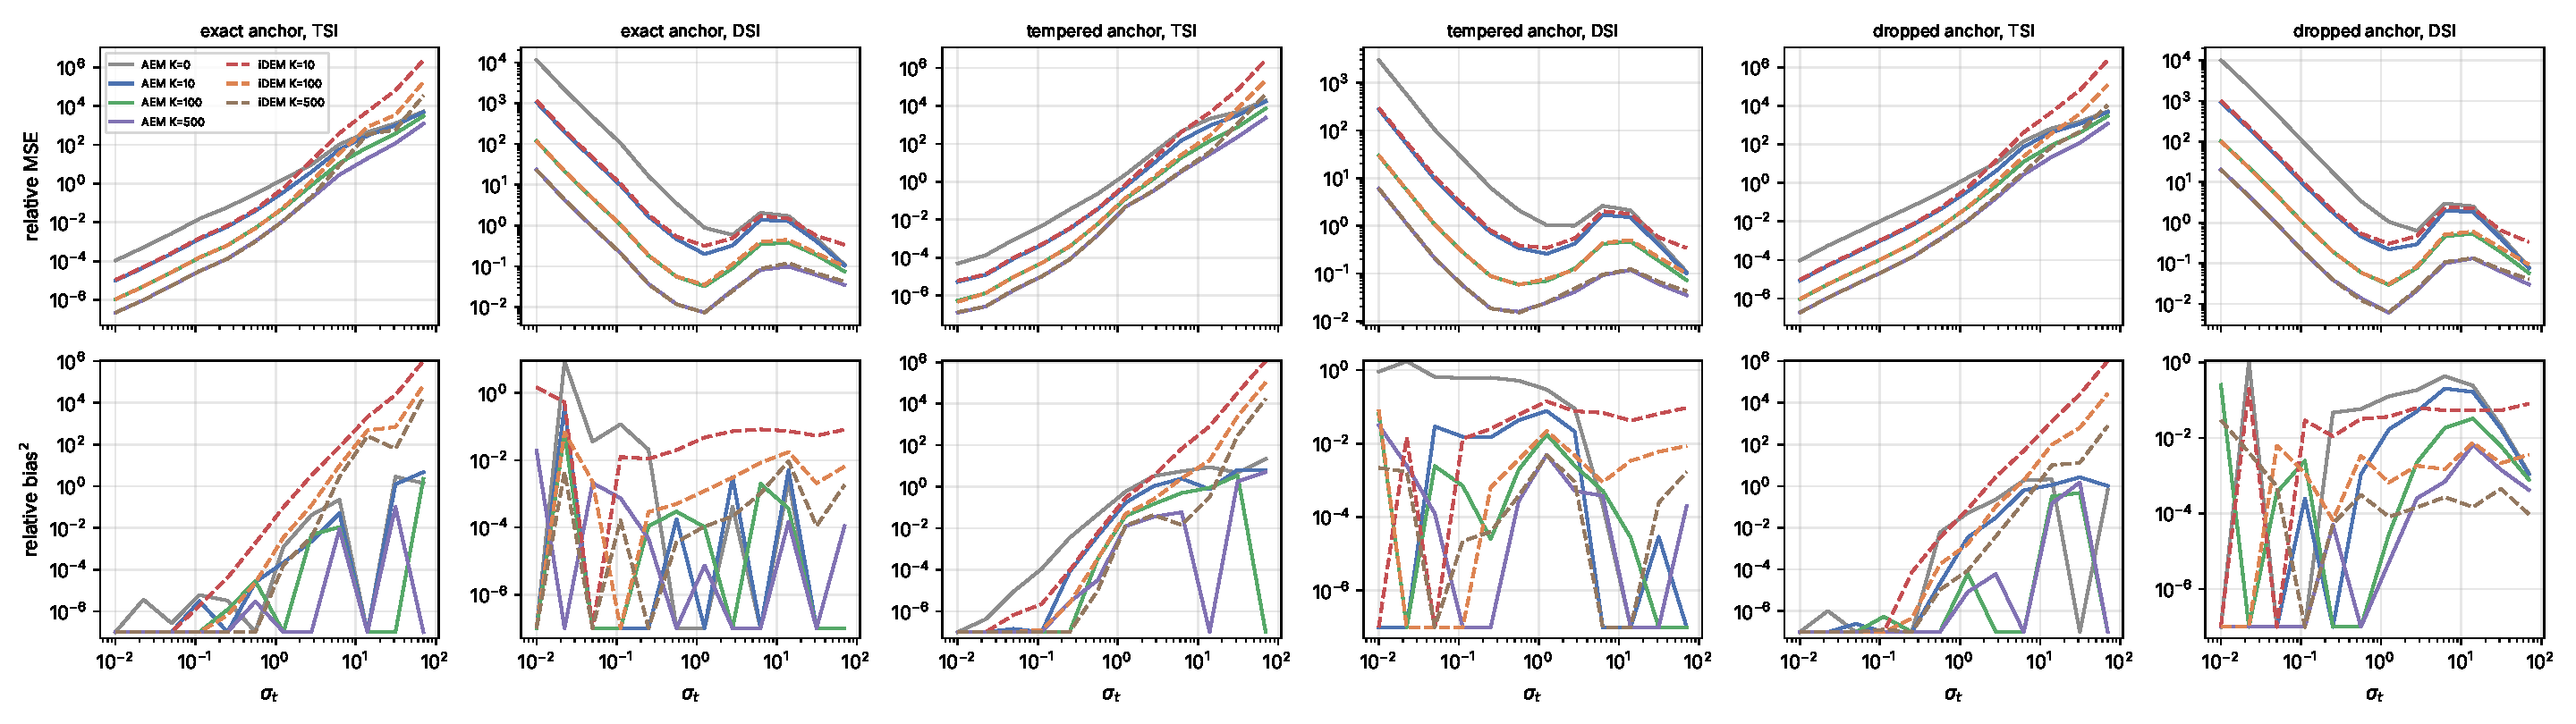
\includegraphics[width=\textwidth]{fig_estimator_gmm40.pdf}
\caption{\textbf{Estimator study on GMM-40.} Relative MSE (top) and debiased relative squared bias (bottom) of the noised-score target against $\sigma_t$, for iDEM (dashed) and AEM (solid) with TSI or DSI test functions. Columns use exact anchors (left), anchors from a tempered target (centre) and anchors from a target missing half of its modes (right). With exact anchors AEM is unbiased for every $K$, including $K=0$. iDEM's bias grows by orders of magnitude with $\sigma_t$.}
\label{fig:estimator}
\end{figure*}

% -------------------------------------------------------------
\subsection{Training samplers (Q2)}
\label{sec:exp-training}
We train on three targets of increasing dimension: GMM-40 ($d=2$), a 10-component Gaussian mixture in $d=16$, and the many-well MW-32 ($d=32$, $2^{16}$ modes).
We compare iDEM, AEM from scratch (\emph{cold}), explore$\to$anchor AEM (iDEM for 20 outer iterations, then anchored targets; the first phase is identical to the iDEM run with the same seed), and explore$\to$anchor AEM with replay proposals (AEM-R).
\Cref{tab:main} reports the final metrics and \cref{fig:curves} the training curves.

\paragraph{iDEM's fixed-point bias is visible, and AEM removes it.}
\Cref{cor:fixed} predicts that iDEM converges to the biased field $b_K$. On MW-32 this bias has a clear signature: the Gaussian coordinates of iDEM samples have variance $4.1\pm0.4$ instead of $1$, and the energy histogram is shifted ($\mathcal{E}$-$\mathcal{W}_1=44.5$). Every AEM variant brings the variance ratio to $1.04$--$1.05$ and lowers $\mathcal{E}$-$\mathcal{W}_1$ by $4$--$29\times$, with a better $\mathcal{W}_2$, at a 1\% higher energy budget.
On GMM-10 ($d=16$) the effect is the same but smaller: the within-mode variance ratio is $1.21$ for iDEM and $1.05$--$1.09$ for AEM, and $\mathcal{E}$-$\mathcal{W}_1$ falls from $1.57$ to $0.29$--$0.62$.
\Cref{fig:marginals} shows the effect directly: iDEM's Gaussian marginals are about twice too wide, its double-well marginals put mass between the wells, and its energy histogram is shifted by about $40$ units. The anchored model matches all three.
These quantities are governed by the within-mode posterior, where the anchor is informative.

\paragraph{In two dimensions there is nothing to fix.}
On GMM-40 all four methods perform similarly ($\mathcal{W}_2$ $4.6$--$5.0$, $\mathcal{E}$-$\mathcal{W}_1$ $0.71$--$0.92$, all 40 modes covered), and most differences are within one standard deviation. This matches the estimator study: in $d=2$, SNIS with $K=100$ is already nearly unbiased at the noise levels that matter. The within-mode variance ratio of $1.7$--$1.9$ is nearly the same for every method, so it reflects the sampler discretization ($\sigma_{\max}/\sigma_{\min}=7000$ with 500 steps) and not the regression target.


\begin{figure*}[t]
\centering
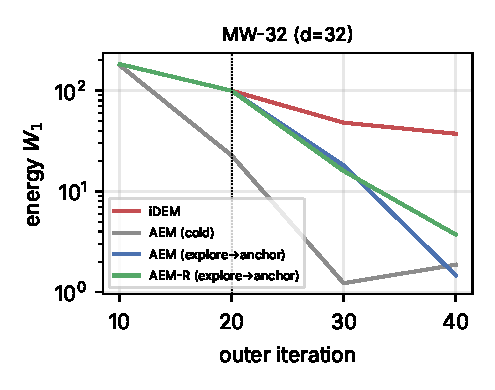
\includegraphics[width=\textwidth]{fig_curves.pdf}
\caption{\textbf{Energy $\mathcal{W}_1$ during training} (mean and min--max over 3 seeds). The dotted line marks the switch from exploration to anchoring in the explore$\to$anchor runs. Before it, those runs coincide with iDEM.}
\label{fig:curves}
\end{figure*}

\begin{figure}[t]
\centering
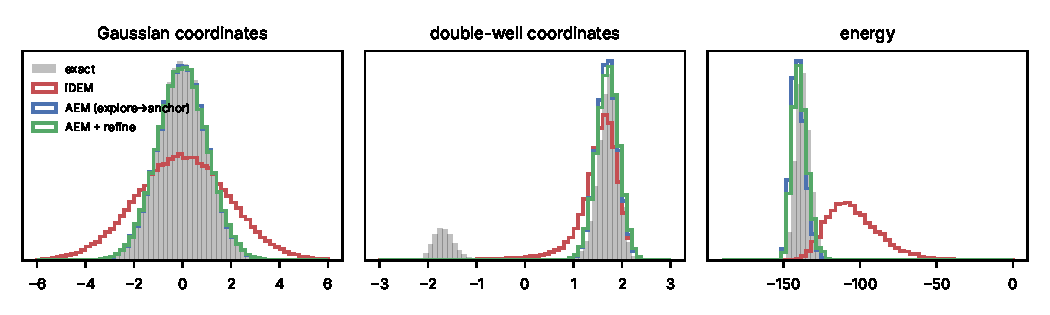
\includegraphics[width=\columnwidth]{fig_mw_marginals.pdf}
\caption{\textbf{MW-32 marginals} (samples pooled over 3 seeds) against exact samples (grey). iDEM's fixed-point bias widens the Gaussian coordinates, smears mass between the wells and shifts the energy distribution. AEM removes these distortions.}
\label{fig:marginals}
\end{figure}

\paragraph{Oracle buffer: testing the fixed point directly.}
To rule out explanations such as short training, the stability caps or the sampler loop, we remove the loop entirely. We train on a \emph{fixed buffer of $10^4$ exact samples} from $\pi$ (\texttt{oracle} mode; rows drawn without replacement), so the buffer law is exactly $\pi$ and \cref{cor:fixed} applies verbatim. We then measure the relative error of the learned score against the exact noised score $\nabla\log p_t$ at $x_t=x_0+\sigma_t\varepsilon$, $x_0\sim\pi$ (\cref{tab:oracle}).
On MW-32 the result is unambiguous. Trained on exact samples, iDEM learns a score whose relative error is $25.0\pm2.6$ at $\sigma_t=1$ and $35.0\pm2.3$ at $\sigma_t=2$ (3 seeds), against $0.140\pm0.003$ and $0.074\pm0.004$ for AEM. Ten times more proposals barely help iDEM: with $K=1000$ (one seed) its error is still $9.8$--$27.6$. This is what one expects from an SNIS bias that decays like $1/K$ with a constant that is exponential in $d$. With a perfect buffer, AEM also gets the mode weights right: in seed 0 the fraction of double-well coordinates in the major well is $0.837$, against a true $0.844$ (iDEM: $0.898$). So the mode-weight deficits of \cref{tab:main} come from the self-generated buffer, as \cref{thm:contraction} predicts, and not from the anchored target.
On GMM-10, where the TSI/DSI combination is exact within each unit-variance component, the two methods learn similar scores at $\sigma_t\ge0.3$ (differences within one standard deviation); AEM is more accurate at $\sigma_t\le0.1$ in the mean.
On the molecular targets we rank the models by held-out denoising loss, which by \cref{prop:diag}(ii) differs between two models by exactly the difference of their score errors (normalized as $\tilde L=\sigma_t^2L/d_{\mathrm{eff}}$; the held-out configurations are disjoint from every seed's buffer). On DW-4 the AEM model has the lower score error at every noise level and in every seed at $\sigma_t\ge0.3$, by a margin that grows from $0.02$ to $10.9$ (\cref{tab:diag}); its samples also have a lower interatomic-distance $\mathcal{W}_1$ in every seed ($0.035$--$0.101$ vs.\ $0.085$--$0.250$). On LJ-13, AEM is better at $\sigma_t\in\{1,2\}$ in all seeds, but slightly worse in the mean at $\sigma_t\le0.3$ (not consistent across seeds), and the gaps are small compared with DW-4. The oracle-trained LJ-13 models of both methods produce some very high-energy samples, so we do not use their sample metrics.



\begin{table*}[t]
\centering
\caption{\textbf{Sampler quality on the synthetic targets} (mean $\pm$ sample std over 3 seeds; $80$ outer iterations; lower is better, except that the variance ratio should be $1$). All methods use the same budget and target function. The variance ratio measures within-mode spread (truth $=1$). Bold marks the best mean in each column (for the variance ratio, the closest to $1$). MMD is the unbiased estimate of MMD$^2$. Mode TV is the total-variation distance between empirical and true mode occupancies (GMM-10: the 10 components; MW-32: the 16 sign patterns of the first four double-well coordinates).}
\label{tab:main}
\small
\begin{tabular}{lccccc}
\toprule
Method & $\mathcal{W}_2$ & $\mathcal{E}$-$\mathcal{W}_1$ & MMD & mode TV & var.\ ratio \\
\midrule
\multicolumn{6}{l}{\textbf{GMM-10 ($d{=}16$)}}\\
iDEM & \textbf{11.6{\scriptsize$\pm$5.6}} & 0.87{\scriptsize$\pm$0.22} & \textbf{0.0138{\scriptsize$\pm$0.018}} & \textbf{0.173{\scriptsize$\pm$0.18}} & 1.12{\scriptsize$\pm$0.027} \\  % n=2
AEM (cold) & 20{\scriptsize$\pm$2} & \textbf{0.125{\scriptsize$\pm$0.079}} & 0.0981{\scriptsize$\pm$0.033} & 0.623{\scriptsize$\pm$0.11} & \textbf{1.02{\scriptsize$\pm$0.013}} \\  % n=2
AEM (explore$\to$anchor) & 14.6{\scriptsize$\pm$3.5} & 0.426{\scriptsize$\pm$0.098} & 0.0309{\scriptsize$\pm$0.021} & 0.286{\scriptsize$\pm$0.18} & 1.06{\scriptsize$\pm$0.013} \\  % n=2
AEM (explore$\to$anchor) + refine & 13.6{\scriptsize$\pm$5} & 0.415{\scriptsize$\pm$0.19} & 0.0258{\scriptsize$\pm$0.027} & 0.275{\scriptsize$\pm$0.2} & 1.06{\scriptsize$\pm$0.026} \\  % n=2
\midrule
\multicolumn{7}{l}{\textbf{MW-32 ($d{=}32$)}}\\
iDEM & 7.74{\scriptsize$\pm$0.17} & 36.4{\scriptsize$\pm$1.5} & \textbf{0.0371{\scriptsize$\pm$0.0048}} & \textbf{0.434{\scriptsize$\pm$0.04}} & 3.67{\scriptsize$\pm$0.22} & 0.974{\scriptsize$\pm$0.0025} \\  % n=2
AEM (cold) & 6.78{\scriptsize$\pm$nan} & \textbf{0.523{\scriptsize$\pm$nan}} & 0.173{\scriptsize$\pm$nan} & 0.481{\scriptsize$\pm$nan} & 1.05{\scriptsize$\pm$nan} & 0.925{\scriptsize$\pm$nan} \\  % n=1
AEM (explore$\to$anchor) & \textbf{6.21{\scriptsize$\pm$0.0051}} & 2.68{\scriptsize$\pm$0.2} & 0.1{\scriptsize$\pm$0.0021} & 0.481{\scriptsize$\pm$0} & \textbf{1.03{\scriptsize$\pm$0.014}} & 1{\scriptsize$\pm$0} \\  % n=2
AEM (explore$\to$anchor) + refine & 6.23{\scriptsize$\pm$0.056} & 1.83{\scriptsize$\pm$0.88} & 0.102{\scriptsize$\pm$0.00041} & 0.481{\scriptsize$\pm$0} & 1.04{\scriptsize$\pm$0.036} & 1{\scriptsize$\pm$0} \\  % n=2
\bottomrule

\end{tabular}
\end{table*}

\begin{table}[t]
\centering
\caption{\textbf{Molecular targets} (mean $\pm$ sample std over 3 seeds; $40$ outer iterations for DW-4, $30$ for LJ-13; EGNN score network). $\mathcal{E}$-$\mathcal{W}_1$: energy-histogram distance; tr: after removing model samples whose energy exceeds the $99.9\%$ quantile of the reference energies (their fraction is in the last column; the reference itself has $0.1\%$); $d$-$\mathcal{W}_1$: $\mathcal{W}_1$ between pooled interatomic distances. Bold marks the best mean per column.}
\label{tab:mol}
\footnotesize
\setlength{\tabcolsep}{3pt}
\begin{tabular}{lcccc}
\toprule
Method & $\mathcal{E}$-$\mathcal{W}_1$ & $\mathcal{E}$-$\mathcal{W}_1^{\mathrm{tr}}$ & $d$-$\mathcal{W}_1$ & frac.\ high-$\mathcal{E}$ \\
\midrule
\multicolumn{5}{l}{\textbf{DW-4 ($d{=}8$)}}\\
iDEM & 1.87{\scriptsize$\pm$0.04} & 0.844{\scriptsize$\pm$0.39} & 0.224{\scriptsize$\pm$0.22} & 0.00224{\scriptsize$\pm$0.0038} \\  % n=3
AEM (explore$\to$anchor) & \textbf{1.85{\scriptsize$\pm$0.008}} & \textbf{0.332{\scriptsize$\pm$0.017}} & \textbf{0.0593{\scriptsize$\pm$0.036}} & \textbf{-5.65e-05{\scriptsize$\pm$0.0001}} \\  % n=2
AEM (explore$\to$anchor) + refine & 1.87{\scriptsize$\pm$0.0013} & 0.635{\scriptsize$\pm$0.16} & 0.142{\scriptsize$\pm$0.13} & 0.000561{\scriptsize$\pm$0.00096} \\  % n=2
\bottomrule

\end{tabular}
\end{table}

% -------------------------------------------------------------
\subsection{Where anchoring fails (Q3)}
\label{sec:exp-ablation}
The same table shows the price of anchoring, and it is the one \cref{thm:contraction} predicts.
When no proposal can reach a mode (high noise, high dimension), $M_t$ is huge and the contraction factor $1-\epsilon_K$ is close to one. The target then follows the buffer: AEM keeps the modes and mode weights the buffer has, and it does not discover new ones.
Started from scratch, AEM inherits whichever modes the first, essentially random, buffers found. On GMM-10 it covers $5$ of $10$ modes (mode TV $0.65$), against $8$ for iDEM (mode TV $0.21$), and its $\mathcal{W}_2$ and MMD are worse accordingly. On MW-32 it occupies the minor wells less evenly than iDEM.
iDEM explores better precisely \emph{because} its target is biased. When SNIS collapses onto the proposal closest to a mode, the resulting field points every noised point towards its nearest low-energy region, which spreads mass across basins whatever the buffer contains.

Exploring first and anchoring afterwards recovers most of iDEM's coverage. On GMM-10 the explore$\to$anchor run keeps all 8 modes iDEM found and still halves $\mathcal{E}$-$\mathcal{W}_1$. It does not recover iDEM's mode-weight accuracy (mode TV $0.35$ vs.\ $0.21$).
Replay proposals were designed to correct mode weights through the energy (\cref{sec:replay}). In our runs they gave the best variance ratio and $\mathcal{W}_2$ on MW-32, but they did not close the mode-weight gap. Used \emph{without} an anchor from the start, they collapse onto the buffer's modes even faster (2 of 10 modes on GMM-10 after 10 iterations; \cref{app:extra}).

The overall picture is consistent. Anchoring makes the target unbiased exactly where the anchor is informative, and it corrects iDEM's systematic within-mode distortion. Mode discovery is a separate problem, and the bias that hurts iDEM's within-mode accuracy is what helps its exploration.
A sampler that wants both needs an exploration mechanism that does not rely on biased targets, such as tempering or annealing across noise levels. Anchoring can be combined with such mechanisms.


\section{Conclusion}
\label{sec:conclusion}
Energy-matching samplers with self-normalized targets, such as iDEM, regress onto Monte Carlo targets whose population minimizer ignores the buffer, so the target distribution is not a fixed point of their training. We showed how to measure this inconsistency from reference samples alone, found it to be large on the standard molecular benchmarks, and removed it by putting back the one exact posterior sample every training pair already contains. The fix costs one line of code and one energy evaluation, and it comes with unbiasedness, variance and contraction guarantees.
Our experiments also separate two effects that are usually measured together. A consistent target fixes the within-mode distribution and the learned score; it does not discover modes, and on our molecular runs it did not by itself give better samplers. Successors with bootstrapped targets, and the original implementations of iEFM and CVSI, can be checked the same way; we tested only our implementations of their target forms. We suggest that new energy-matching objectives report the consistency test of \cref{prop:diag}, which is cheap, and that consistent targets be paired with exploration that does not rely on biased estimators (tempering, annealed importance sampling, parallel chains across noise levels).
\paragraph{Limitations.}
Our targets have at most 39 dimensions; training budgets are short ($3000$--$8000$ steps), with 3 seeds and no per-method tuning, and several comparisons are within one standard deviation. LJ-13 uses a smaller network and sampler grid. The molecular test and oracle runs are relative to MALA references, which may miss isolated basins. Larger budgets may change the ranking on mode-level and molecular metrics. We compare only with iDEM in training.


\section*{Impact Statement}
This paper presents work whose goal is to advance the field of machine learning, specifically sampling from unnormalized densities as used in Bayesian inference and molecular simulation. We do not foresee societal consequences that need to be highlighted here beyond those of the field in general.

\bibliography{refs}
\bibliographystyle{icml2026}

\newpage
\appendix
\onecolumn
\section{Proofs}
\label{app:proofs}

Throughout, $x_t$ and $t$ are fixed. We write $\pi_t$ for the posterior $\pi_t(\cdot\mid x_t)$, $q$ for the proposal, and $\bar w=\pi_t/q$ for the normalized importance weight, so that $\mathbb{E}_q[\bar w]=1$. The unnormalized weights $w=\tilde\pi\,\mathcal{N}(x_t;\cdot,\sigma_t^2I)/q$ used in \eqref{eq:aem} differ from $\bar w$ by a factor that does not depend on the particle, and that factor cancels after self-normalization. We may therefore use $\bar w$ throughout. Let $Y=(y_0,\dots,y_K)$ and $W_j=\bar w(y_j)/\sum_{k=0}^K\bar w(y_k)$.

\subsection{Proof of \cref{thm:unbiased}}
Define the extended distribution on $\{0,\dots,K\}\times(\mathbb{R}^d)^{K+1}$
\[
\Gamma(j,Y)=\frac{1}{K+1}\,\pi_t(y_j)\prod_{k\neq j}q(y_k).
\]
Under $\Gamma$, $J$ is uniform and, given $J=j$, the particle $y_j$ is a posterior draw and the others are independent proposals. By exchangeability, the law of the unordered particle set under $\Gamma$ is the same as the law of the AEM particle system, in which the posterior draw always sits at index $0$. Since $\widehat A_K$ is a symmetric function of the particles, its law is the same under both.
Marginalizing $J$,
\[
\Gamma(Y)=\prod_{k=0}^K q(y_k)\cdot\frac{1}{K+1}\sum_{j=0}^K\bar w(y_j),
\]
so $\Gamma(J=j\mid Y)=W_j$. Therefore
\[
\mathbb{E}_\Gamma[g(y_J)\mid Y]=\sum_j W_j\,g(y_j)=\widehat A_K(Y),
\]
and by the tower property $\mathbb{E}[\widehat A_K]=\mathbb{E}_\Gamma[g(y_J)]=\mathbb{E}_{\pi_t}[g]$, because $y_J\sim\pi_t$ under $\Gamma$.
For the covariance, the law of total covariance gives
$\mathrm{Cov}_\Gamma[g(y_J)]=\mathrm{Cov}[\mathbb{E}(g(y_J)\mid Y)]+\mathbb{E}[\mathrm{Cov}(g(y_J)\mid Y)]\succeq\mathrm{Cov}[\widehat A_K]$, and $\mathrm{Cov}_\Gamma[g(y_J)]=\mathrm{Cov}_{\pi_t}[g]$.
None of these steps uses the specific form of $q$. The result holds for any proposal whose support contains that of $\pi_t$, and for any $K\ge0$. \hfill$\square$

\subsection{Proof of \cref{cor:fixed}}
The AEM loss is $\mathbb{E}\,\lambda_t\|s(x_t,t)-\widehat A_K\|^2$. Over all measurable $s$, its minimizer is $s(x,t)=\mathbb{E}[\widehat A_K\mid x_t=x]$. When $x_0\sim\pi$, the conditional law of $x_0$ given $x_t$ is $\pi_t(\cdot\mid x_t)$, so \cref{thm:unbiased} applies with $g$ from TSI or DSI, and both identities \eqref{eq:tsi}--\eqref{eq:dsi} give $\nabla\log p_t(x)$. For iDEM, the target $\widehat S_K$ is a function of $(x_t,y_{1:K})$ alone, and $y_{1:K}\mid x_t\sim q^{\otimes K}$ whatever the buffer law. Hence the minimizer is $b_K(x,t)=\mathbb{E}_{q^{\otimes K}}[\widehat S_K(x)]$ for every $\rho$. \hfill$\square$

\subsection{Proof of \cref{prop:refine}}
Fix $R$ and consider one chain $x\sim\pi$, together with $x_t\mid x\sim\mathcal{N}(x,\sigma^2 I)$ (for the projected molecular targets, noise lives in the same subspace as $\pi$). The pair $(x,x_t)$ has density $\pi(x)\mathcal{N}(x_t;x,\sigma^2I)$, so $x\mid x_t\sim\pi_t(\cdot\mid x_t)$ exactly: the noising step is an exact Gibbs draw of $x_t$ given $x$.
Given $x_t$, the proposal $q(\cdot\mid x_t,R)$ does not depend on $x$, and $R$ is fixed. Under $x\sim\pi_t(\cdot\mid x_t)$, \cref{thm:unbiased} (with $K\ge1$ and the same particle system, $y_0=x$) shows that the unordered set $\{x,y_1,\dots,y_K\}$ has the exchangeable law $\Gamma$ of its proof, and the index selected with probability $W_j\propto\bar w(y_j)$ satisfies $\Gamma(J=j\mid Y)=W_j$. Hence the selected particle $x'=y_J$ is distributed as $\pi_t(\cdot\mid x_t)$: step (2) is the i-SIR kernel, which is reversible with respect to $\pi_t(\cdot\mid x_t)$ \citep{andrieu2010particle}. Therefore the pair $(x',x_t)$ has the same joint law $\pi(x)\mathcal{N}(x_t;x,\sigma^2I)$ as $(x,x_t)$, and in particular $x'\sim\pi$. The noise level $\sigma$ may be drawn from any fixed law independent of $x$, and the claim holds conditionally on $\sigma$.
For a block $S$ with fixed $R$, the chains in $S$ are independent given $R$ under $\pi^{\otimes N}$, and each is updated by a kernel that depends only on $R$, its own noise and its own proposals. So $\mathcal{P}_R$ leaves $\pi^{\otimes|S|}$ invariant for every $R$. If $x^{1:N}\sim\pi^{\otimes N}$ then $x^S$ and $x^{R}$ are independent, so conditioning on $x^R$ and applying $\mathcal{P}_{x^R}$ to $x^S$ yields $(x'^{S},x^{R})\sim\pi^{\otimes N}$. Visiting the blocks one after another, each with a reference set drawn from chains outside the current block (possibly after earlier blocks have been updated, which keeps the law $\pi^{\otimes N}$), preserves $\pi^{\otimes N}$ at every stage. \hfill$\square$

\paragraph{Remark.} The proposition concerns an exact buffer. For a buffer drawn from the model, whose law $\rho\neq\pi$, the same construction gives a kernel with $\pi^{\otimes N}$ as invariant law, so repeated sweeps push the buffer towards $\pi$ if the kernel is ergodic. We do not prove a rate here. Our implementation also draws the reference set as a random subset of 512 of the other chains, which is a function of $x^R$ only and so does not affect the argument.

\subsection{A closed-form iDEM counterexample}
\label{app:idem-bias}
Let $\pi=\mathcal{N}(0,I_d)$ and $g(y)=-\nabla\mathcal{E}(y)=-y$ (TSI). The true noised score is $-x_t/(1+\sigma_t^2)$. With $K=1$, SNIS returns $g(y_1)$ with $y_1\sim\mathcal{N}(x_t,\sigma_t^2I)$, so
\[
b_1(x_t)=-x_t,\qquad b_1(x_t)-\nabla\log p_t(x_t)=-\frac{\sigma_t^2}{1+\sigma_t^2}\,x_t .
\]
The relative bias goes to $1$ as $\sigma_t$ grows. In contrast, the anchored estimator with $K=1$ is $(\bar w(x_0)(-x_0)+\bar w(y_1)(-y_1))/(\bar w(x_0)+\bar w(y_1))$, and it is exactly unbiased by \cref{thm:unbiased}. For $K>1$, the SNIS bias has the classical expansion $b_K-\bar g=-\frac1K\mathbb{E}_q[\bar w^2(g-\bar g)]+O(K^{-2})$~\citep{owen2013monte}. The leading term is nonzero here, and for this Gaussian $\mathbb{E}_q[\bar w^2]$ grows like $(1+\sigma_t^2)^{d}/(1+2\sigma_t^2)^{d/2}$, so for fixed $K$ the bias grows rapidly with $\sigma_t$ and $d$. We verify this numerically in \cref{sec:exp-estimator}.

\subsection{Proof of \cref{thm:contraction}}
\emph{Identity.} Let $y_0\sim\mu$ and $y_{1:K}\overset{\text{iid}}{\sim}q$. Define $J\mid Y\sim\mathrm{Cat}(W)$. Then $\widehat A_K=\mathbb{E}[g(y_J)\mid Y]$, so $\mathbb{E}\widehat A_K=\mathbb{E}g(y_J)=(\mu P_K)(g)$, where $P_K(y_0,\cdot)$ is the law of $y_J$. This kernel is the i-SIR kernel. It leaves $\pi_t$ invariant: under $\Gamma$, starting from $y_0\sim\pi_t$, \cref{thm:unbiased} shows $y_J\sim\pi_t$.

\emph{Minorization.} Fix $y_0$ and a measurable set $B$. Write $S=\sum_{k=2}^K\bar w(y_k)$. Dropping the anchor term and using symmetry in $y_{1:K}$,
\[
P_K(y_0,B)\;\ge\;K\,\mathbb{E}\!\left[\frac{\bar w(y_1)\mathbf 1_B(y_1)}{\bar w(y_0)+\bar w(y_1)+S}\right]
\;\ge\;K\,\mathbb{E}\big[\bar w(y_1)\mathbf 1_B(y_1)\big]\;\mathbb{E}\!\left[\frac{1}{2M_t+S}\right],
\]
because $\bar w\le M_t$ and $y_1$ is independent of $S$. Now $\mathbb{E}_q[\bar w\mathbf 1_B]=\pi_t(B)$, and Jensen's inequality for the convex map $u\mapsto(2M_t+u)^{-1}$ with $\mathbb{E}S=K-1$ gives $\mathbb{E}[(2M_t+S)^{-1}]\ge(2M_t+K-1)^{-1}$. Hence $P_K(y_0,\cdot)\ge\epsilon_K\pi_t(\cdot)$ with $\epsilon_K=K/(K-1+2M_t)$.

\emph{Contraction.} Write $P_K=\epsilon_K\Pi+(1-\epsilon_K)R$, where $\Pi(y,\cdot)=\pi_t$ and $R$ is a Markov kernel. Then $(\mu-\pi_t)P_K=(1-\epsilon_K)(\mu-\pi_t)R$, since $(\mu-\pi_t)\Pi=0$ and $\pi_tP_K=\pi_t$. For bounded $g$, this yields $|(\mu P_K-\pi_t)g|\le(1-\epsilon_K)\,2\,\mathrm{TV}(\mu,\pi_t)\|g\|_\infty$. Applied coordinatewise, the bound holds for vector-valued $g$ with $\|g\|_\infty=\sup_y\|g(y)\|_\infty$. Iterating $n$ times gives the factor $(1-\epsilon_K)^n$. \hfill$\square$

\begin{remark}[Unbounded $g$]
The TSI and DSI test functions are unbounded. The same argument goes through in a weighted norm $\|f\|_V=\sup|f|/V$ whenever $P_K$ satisfies a drift condition for $V$. We state the bounded case for clarity: the qualitative message (contraction factor $1-\epsilon_K$) is unchanged.
\end{remark}

\section{Experimental details}
\label{app:exp}

\paragraph{Targets.}
\emph{GMM-40} ($d=2$) is a mixture of 40 equal-weight isotropic unit-variance Gaussians whose means are drawn uniformly from $[-40,40]^2$~\citep{midgley2023flow}.
\emph{GMM-10} ($d=16$) is a mixture of 10 equal-weight unit-variance Gaussians with means uniform in $[-10,10]^{16}$.
\emph{MW-32} is the many-well energy $\mathcal{E}(x)=\sum_{i=1}^{16}\big(x_{2i-1}^4-6x_{2i-1}^2-0.5x_{2i-1}+0.5x_{2i}^2\big)$ with $2^{16}$ modes~\citep{midgley2023flow}. Each double-well coordinate puts about $84\%$ of its mass in the right-hand well.
All three targets admit exact samples, and the Gaussian mixtures also admit closed-form noised scores and exact posterior draws. These are used for the estimator study. For MW-32 the noised score factorizes over coordinates and is computed by quadrature.

\paragraph{Noise schedule and network.}
We use the VE schedule $\sigma_t=\sigma_{\min}(\sigma_{\max}/\sigma_{\min})^t$ with $\sigma_{\min}=0.01$ and $\sigma_{\max}=70$ (GMM-40), $20$ (GMM-10) and $3$ (MW-32).
The score network is an MLP with four hidden layers of width 256, SiLU activations and a sinusoidal time embedding. It is preconditioned so that the network predicts $\sigma_t\,s(x,t)$.
For stability we cap the norm of $\sigma_t\times$(target) and of $\sigma_t\times$(sampler score) at $10\sqrt d$, and we clip per-particle energy gradients at norm $10^3$ (GMM-40). These rules are identical for all methods.

\paragraph{Training protocol.}
Every method uses the same outer/inner loop as iDEM: 40 outer iterations, each with 100 Adam steps (learning rate $5\cdot10^{-4}$, batch 256, gradient clipping at norm 1). Each outer iteration then adds 1000 reverse-SDE samples to a FIFO buffer of size $10^4$. The SDE uses 200 Euler--Maruyama steps for the GMMs and 300 for MW-32 during training, and 500/1000 steps for evaluation.
All methods use $K=100$ proposals and the same test function, the precision-weighted combination $g=\alpha_t g_{\mathrm{TSI}}+(1-\alpha_t)g_{\mathrm{DSI}}$ with $\alpha_t=(1+\sigma_t^2)^{-1}$. In our initial GMM-40 runs with pure TSI targets (before the norm caps above were added), training diverged for both iDEM and AEM. \Cref{sec:exp-estimator} shows the cause: the TSI estimator's relative variance explodes at high noise. We therefore give iDEM the same stabilized target, which makes it a stronger baseline than the original.
\emph{Explore$\to$anchor} runs share their first 20 outer iterations with iDEM (same seed, so identical trajectories) and anchor afterwards. AEM-R additionally uses replay proposals \eqref{eq:replay} with $\alpha=0.5$ and $\tau_{\max}=1$ (GMMs) or $0.5$ (MW-32) in the anchored phase.
AEM evaluates $K+1$ energies per target instead of $K$, a 1\% overhead. AEM-R additionally computes a $B\times K\times B$ log-sum-exp.

\paragraph{Metrics.}
All metrics compare 2000 model samples with 2000 exact samples: exact $\mathcal{W}_2$ (Hungarian matching on 1000 points), $\mathcal{W}_1$ between energy histograms ($\mathcal{E}$-$\mathcal{W}_1$), MMD with a median-heuristic RBF kernel, and the total-variation distance between empirical and true mode occupancies (GMMs: nearest mean; MW-32: the 16 sign patterns of the first four double-well coordinates).
The \emph{variance ratio} measures within-mode spread: $\frac{1}{d}\mathbb{E}\|x-\mu_{\mathrm{nearest}}\|^2$ for the GMMs (truth $1$), and the variance of the Gaussian coordinates for MW-32 (truth $1$).
All experiments ran on 4 CPU cores.


\end{document}
